\section{Analysis}\label{sec:analysis}

\subsection{Experimental Data}
The experimental data consist of events recorded using a LaBr$_3$(Ce) scintillation detector while measuring the gamma-ray spectrum of a $^{152}\mathrm{Eu}$ source. The data contains 6 columns:
\begin{description}
    \item[\texttt{BOARD}:] Identifies the digitizer board that recorded the event.
    \item[\texttt{CHANNEL}:] Identifies the input channel of the digitizer to which the detector signal was connected.
    \item[\texttt{TIMETAG}:] Records the event timestamp as a digitizer clock count, allowing the temporal ordering and timing of events to be determined.
    \item[\texttt{ENERGY}:] Stores the integrated charge measured using a long integration gate, which serves as the primary parameter for constructing the gamma-ray energy spectrum.
    \item[\texttt{ENERGYSHORT}:] Stores the integrated charge measured using a shorter integration gate, providing an additional parameter useful for pulse-shape analysis.
    \item[\texttt{FLAGS}:] Contains hexadecimal status bits encoding additional information about the recorded event.
\end{description}

\subsection{Identification of Prominent Peaks}
We plotted a histogram with 8192 equally spaced bins over the range of the recorded uncalibrated energy. The resulting histogram \cref{fig:spectrum} represents the number of detected events in each bin and provides the experimental gamma-ray spectrum. The obtained histogram contains statistical fluctuations arising from the finite number of recorded events. These fluctuations can produce small local maxima that should not necessarily be interpreted as individual gamma-ray peaks.

\begin{figure}[h]
    \centering
    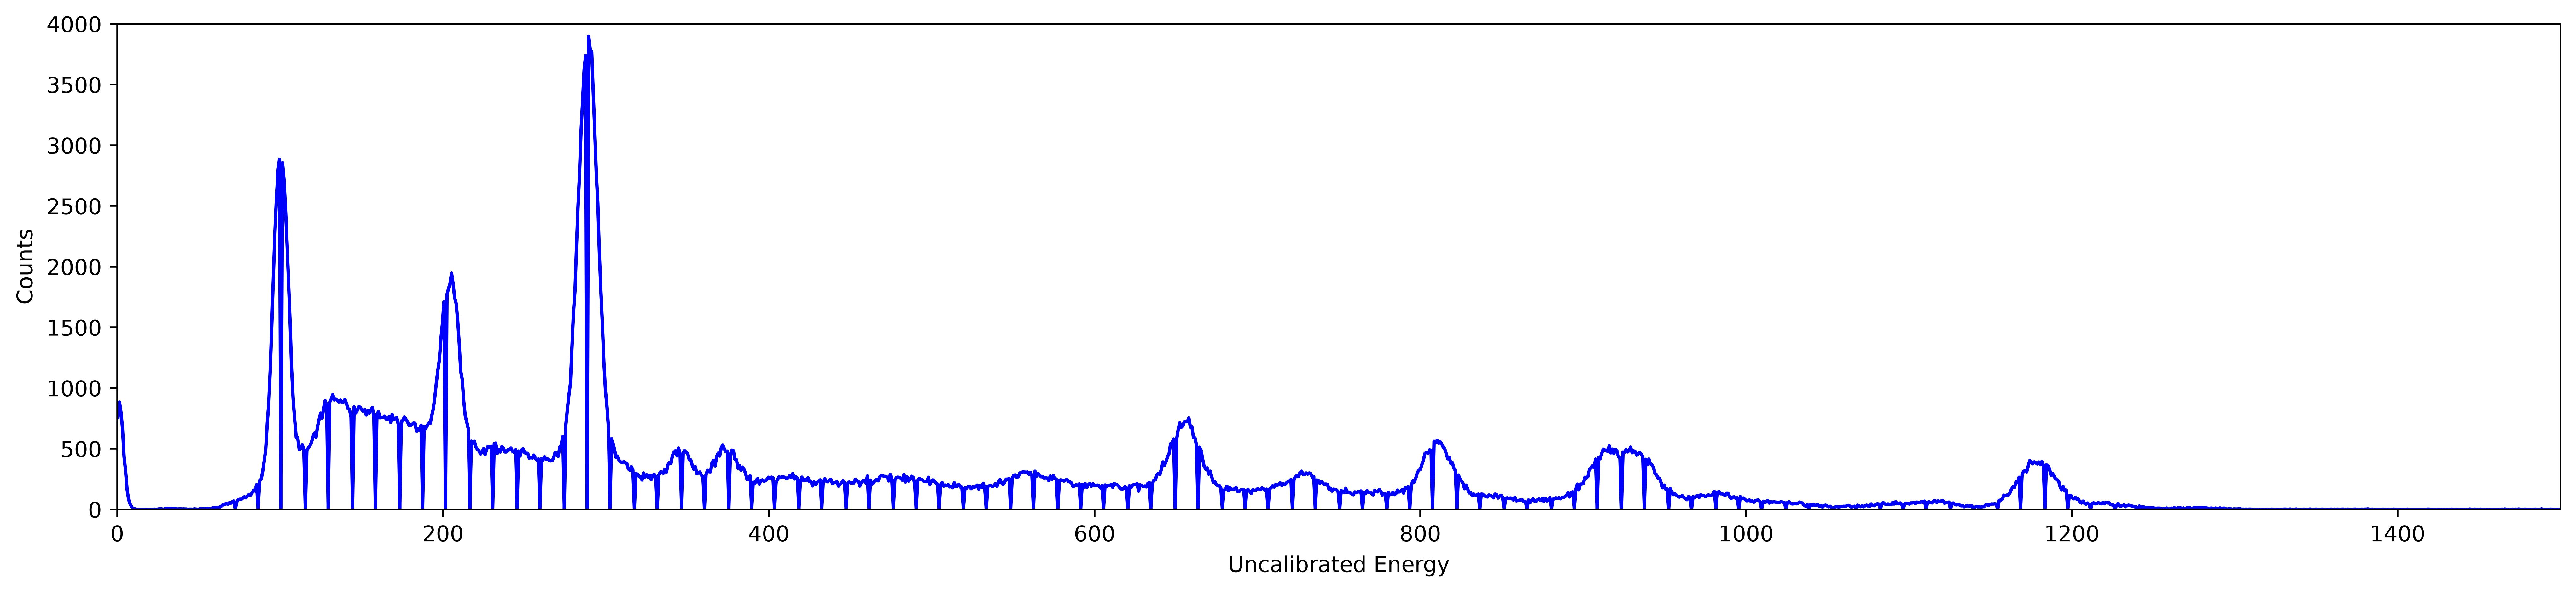
\includegraphics[width=\linewidth]{Images/spectrum.jpg}
	\caption{Histogram with 8192 equally spaced bins over the range of the recorded uncalibrated energy.}
	\label{fig:spectrum}
\end{figure}

To obtain a more stable representation of the spectrum, we applied Gaussian smoothing to the histogram using a one-dimensional Gaussian kernel with standard deviation 5 bins. The smoothing suppresses short-scale statistical fluctuations while retaining the overall structure and locations of the prominent spectral features.

\begin{figure}[h]
    \centering
    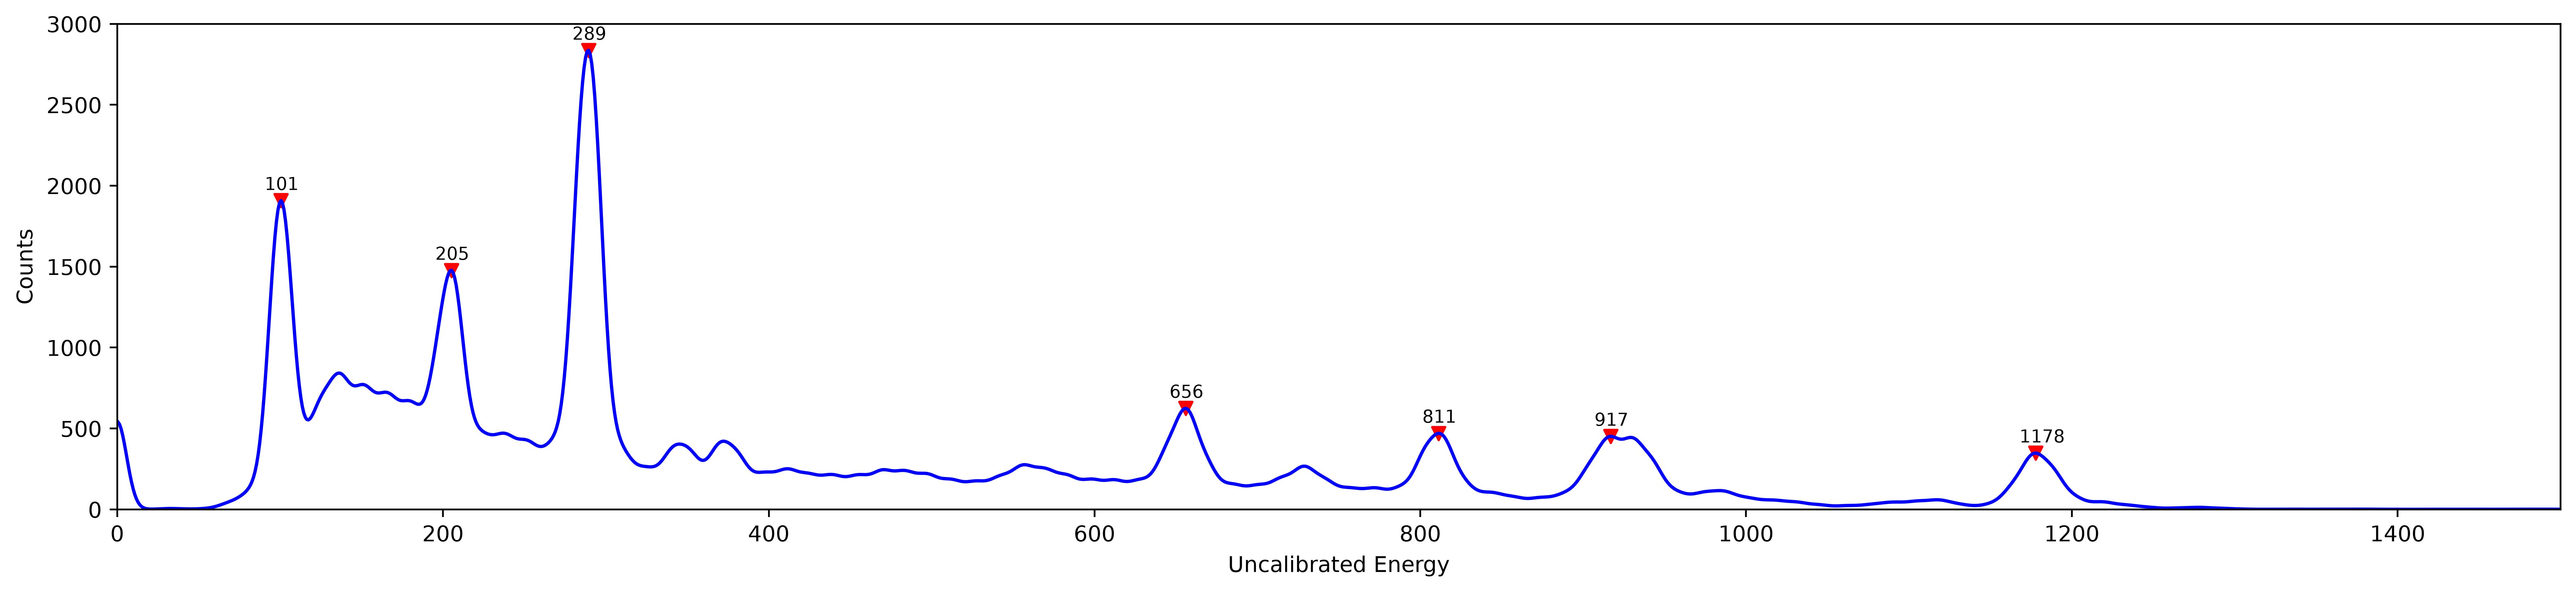
\includegraphics[width=\textwidth]{Images/spectrum_smoothed.jpg}
	\caption{Histogram from \cref{fig:spectrum} smoothed using a Gaussian kernel with standard deviation 5 bins.}
	\label{fig:spectrum smoothed}
\end{figure}

We have identified the peaks at - 100.53, 205.27, 289.44, 656.03, 811.27, 916.94 and 1177.86.

\subsection{Gaussian Fitting of the Detected Peaks}
The peak positions obtained from the detection algorithm provide initial estimates of the peak centres. However, locating the maximum of a discretely sampled histogram does not necessarily provide the most accurate estimate of the underlying peak position. We therefore fitted each detected peak independently using a Gaussian function accompanied by a linear background (assuming the background varies very slowly within the width of the peak):
\begin{equation}
    N(x) = A\exp\left[-\frac{(x-x_0)^2}{2\sigma^2}\right] + a + bx.
    \label{eq:peak fit}
\end{equation}
Here, $A$ represents the peak amplitude, $x_0$ is the Gaussian centre, and $\sigma$ characterises the width of the Gaussian distribution. The parameters $a$ and $b$ describe the local background level and its linear variation across the fitting region.

\begin{figure}[h]
	\centering
	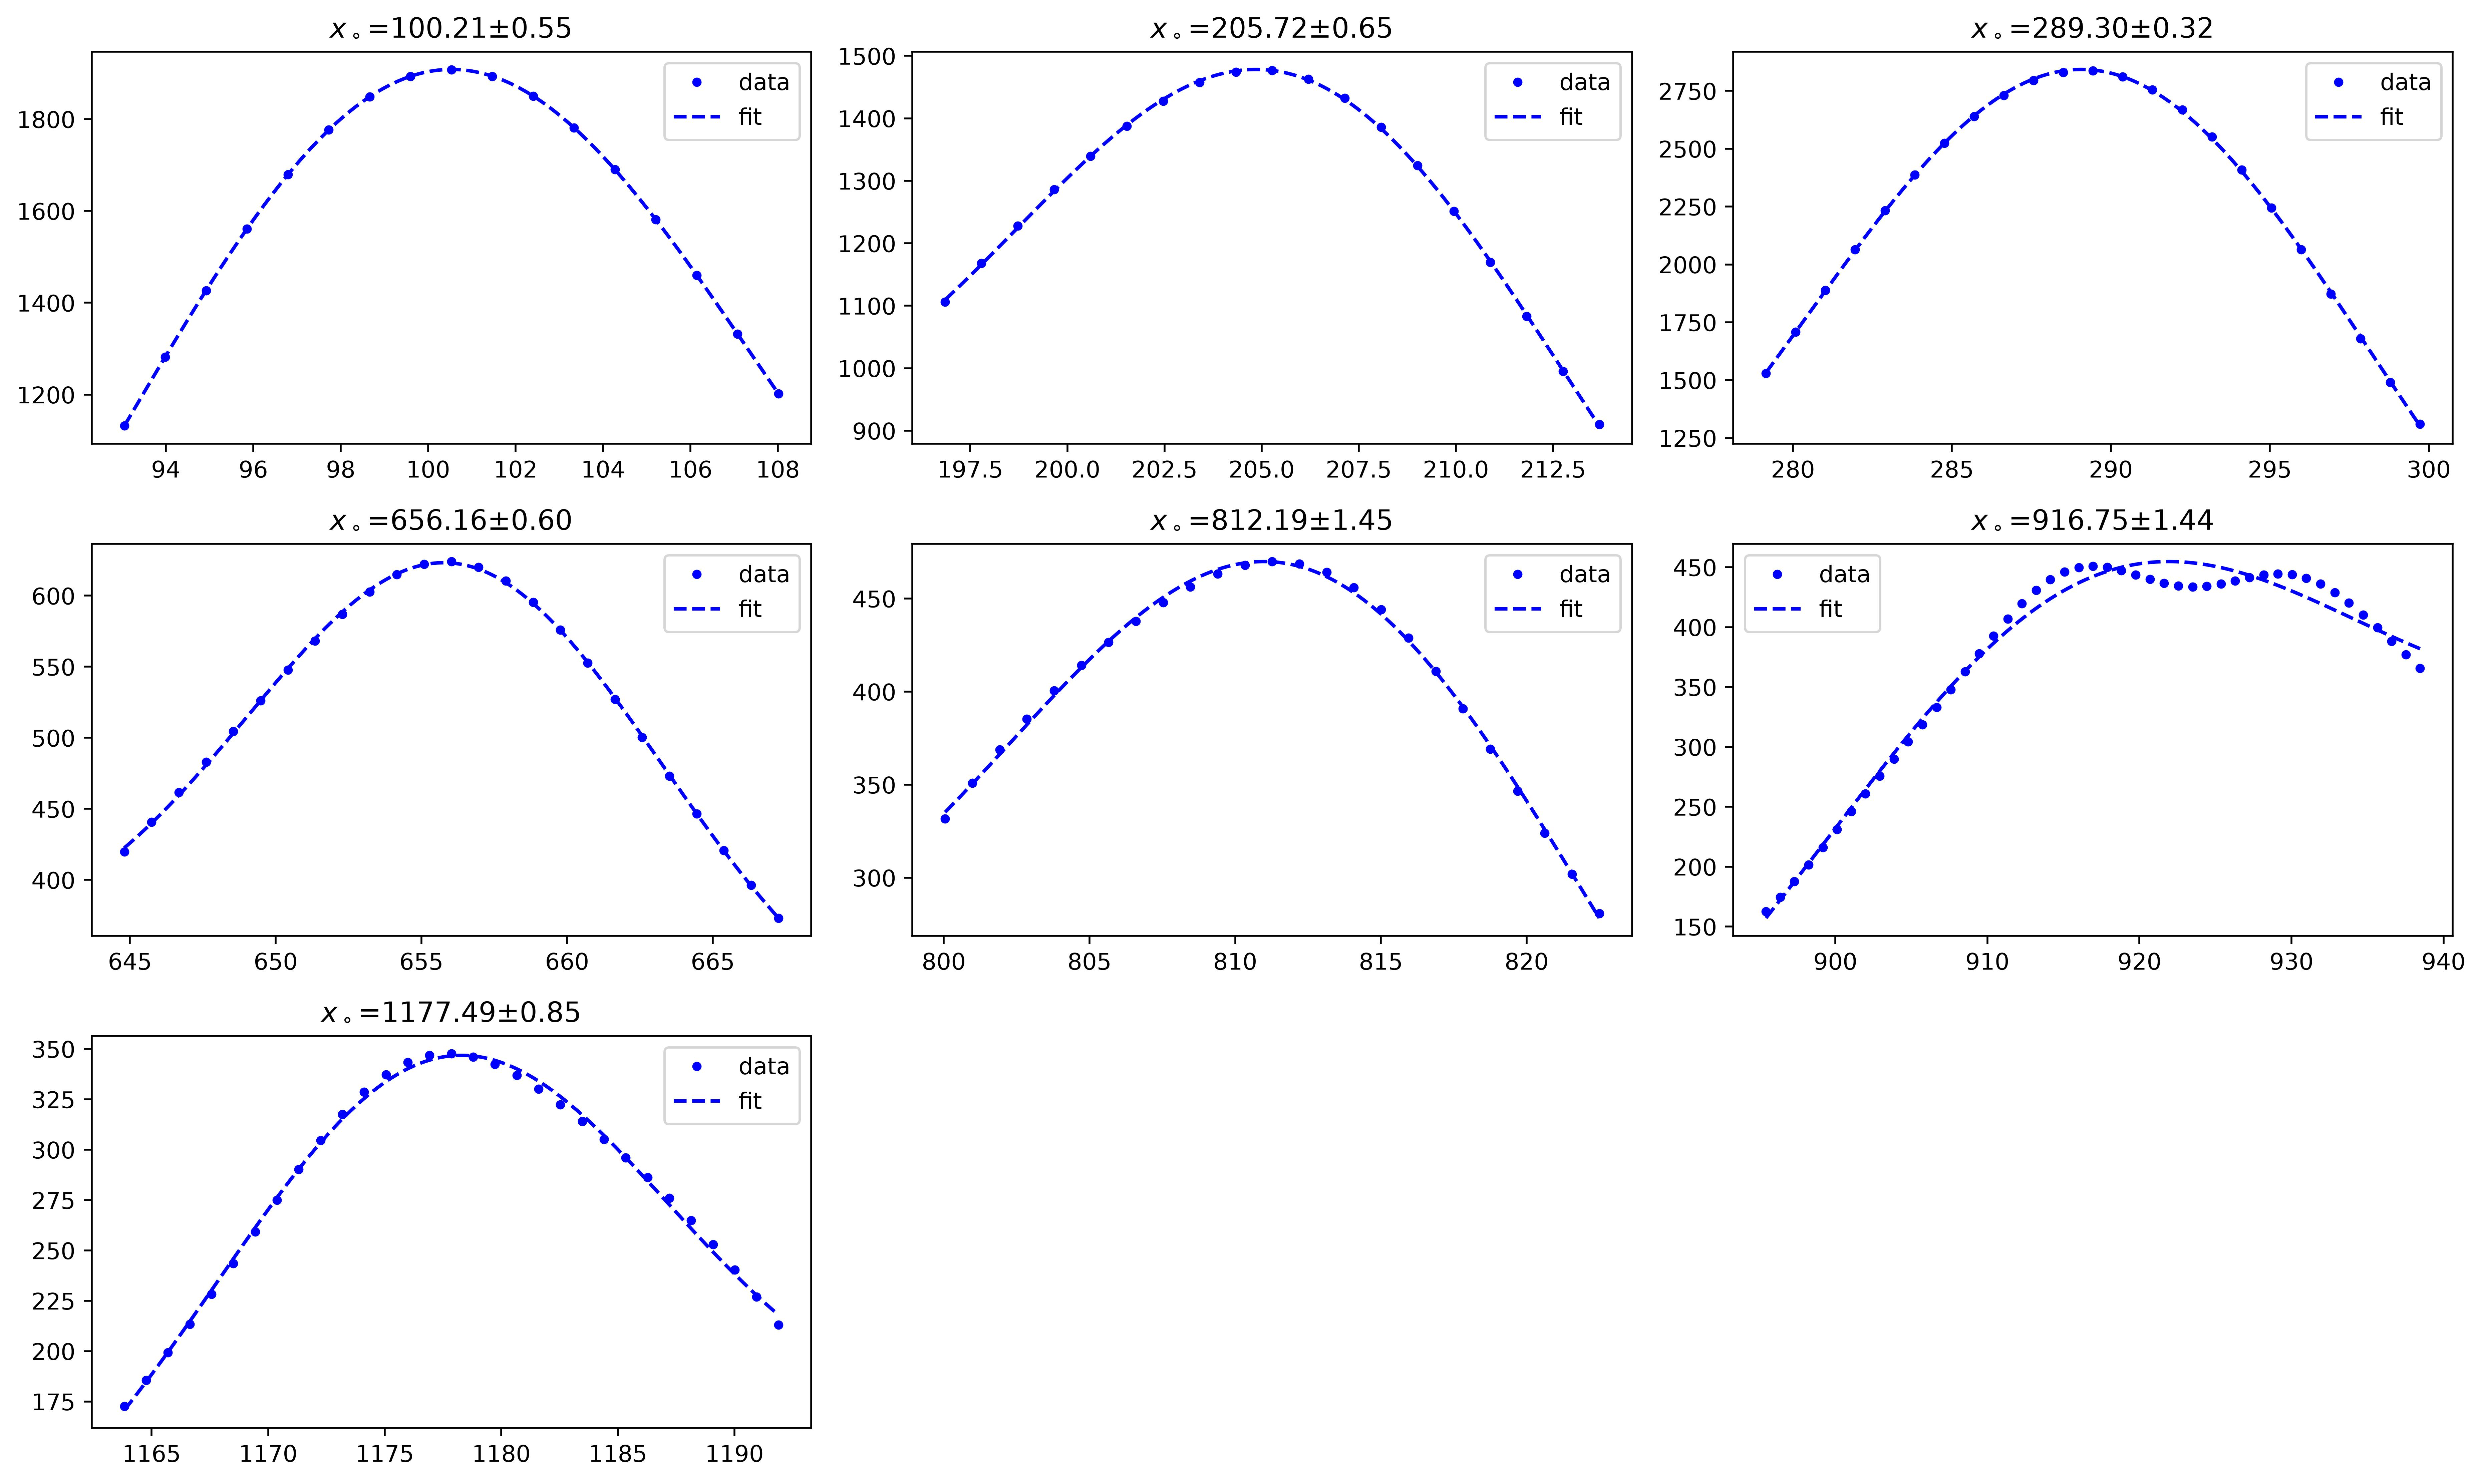
\includegraphics[width=\textwidth]{Images/gaussian_fitting.jpg}
	\caption{Gaussian fit to each peak independently with linear background (\cref{eq:peak fit})}
	\label{fig:gaussian fit}
\end{figure}

\begin{figure}[h]
    \centering
    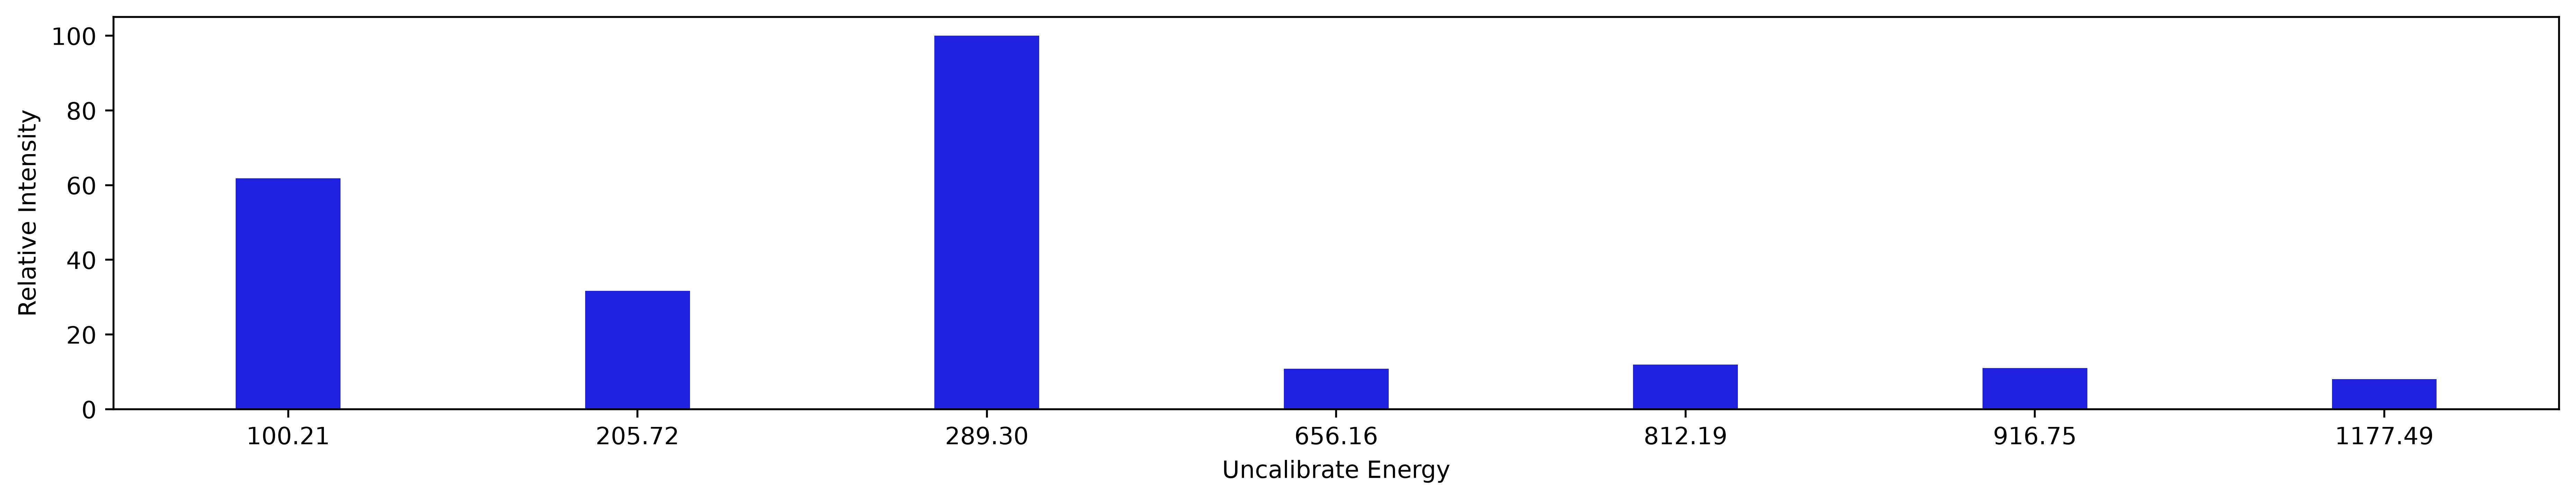
\includegraphics[width=\linewidth]{Images/detected_peaks.jpg}
    \caption{Detected peaks with bar height representing relative intensity determined from the amplitude of \cref{eq:peak fit}.}
    \label{fig:detetcted peaks}
\end{figure}

The resulting fitted peak positions and widths are summarised in \cref{tab:detected peaks}.

\begin{table}[htbp]
    \centering
    \begin{tabular}{c c c c}
        \toprule
        Peak & Position & Peak width & Relative intensity (\%) \\
        \midrule
        1 & 100.21 & 14.50 & 61.81 \\
        2 & 205.72 & 14.11 & 31.71 \\
        3 & 289.30 & 17.77 & 100.00 \\
        4 & 656.16 & 14.21 & 10.84 \\
        5 & 812.19 & 19.81 & 11.93 \\
        6 & 916.75 & 34.62 & 11.01 \\
        7 & 1177.49 & 19.34 & 8.04 \\
        \bottomrule
    \end{tabular}
    \caption{Gaussian fit result of each peak. The peak width is $2\sigma$ and intensity is the amplitude $A$ in \cref{eq:peak fit}. The intensities have been normalised with respect to the largest intensity.}
    \label{tab:detected peaks}
\end{table}

\subsection{Comparison with Reference Gamma-Ray Energies}
After determining the experimental peak positions, we compared the measured spectrum with reference gamma-ray transition energies associated with $^{152}\mathrm{Eu}$ from the \textbf{ENSDF} dataset\cite{ensdf}. The dataset contains all gamma transtitions including metastable states. The lifetime of the metastable states are very small\cite{enwiki:1352528506}. Assuming the source is old enough, we ignored those transitions.

To restrict the comparison to sufficiently prominent reference transitions, we retained only entries having relative intensity greater than 5. This selection yielded 13 candidate reference gamma-ray energies as shown in \cref{tab:actual energies} and \cref{fig:actual energies}.

\begin{table}[htbp]
    \centering
    \begin{tabular}{c c c c}
        \hline
        Peak & Energy (keV) & Relative intensity (\%) & Decay type \\
        \hline
        1 & 121.78  & 100.0000 & EC \\
        2 & 244.70  & 26.46  & EC \\
        3 & 344.28  & 93.20  & $\beta^-$ \\
        4 & 411.12  & 7.84   & $\beta^-$ \\
        5 & 443.96  & 9.91   & EC \\
        6 & 778.90  & 45.31  & $\beta^-$ \\
        7 & 867.38  & 14.82  & EC \\
        8 & 964.06  & 50.86  & EC \\
        9 & 1085.84 & 35.45  & EC \\
        10 & 1089.74 & 6.08   & $\beta^-$ \\
        11 & 1112.08 & 47.90  & EC \\
        12 & 1299.14 & 5.72   & $\beta^-$ \\
        13 & 1408.01 & 73.14  & EC \\
        \hline
    \end{tabular}
    \caption{Reference gamma-ray energies from the \textbf{ENSDF} dataset. EC corresponds to elentron capture. The intensities have been normalised with respect to the largest intensity.}
    \label{tab:actual energies}
\end{table}

\begin{figure}[h]
	\centering
	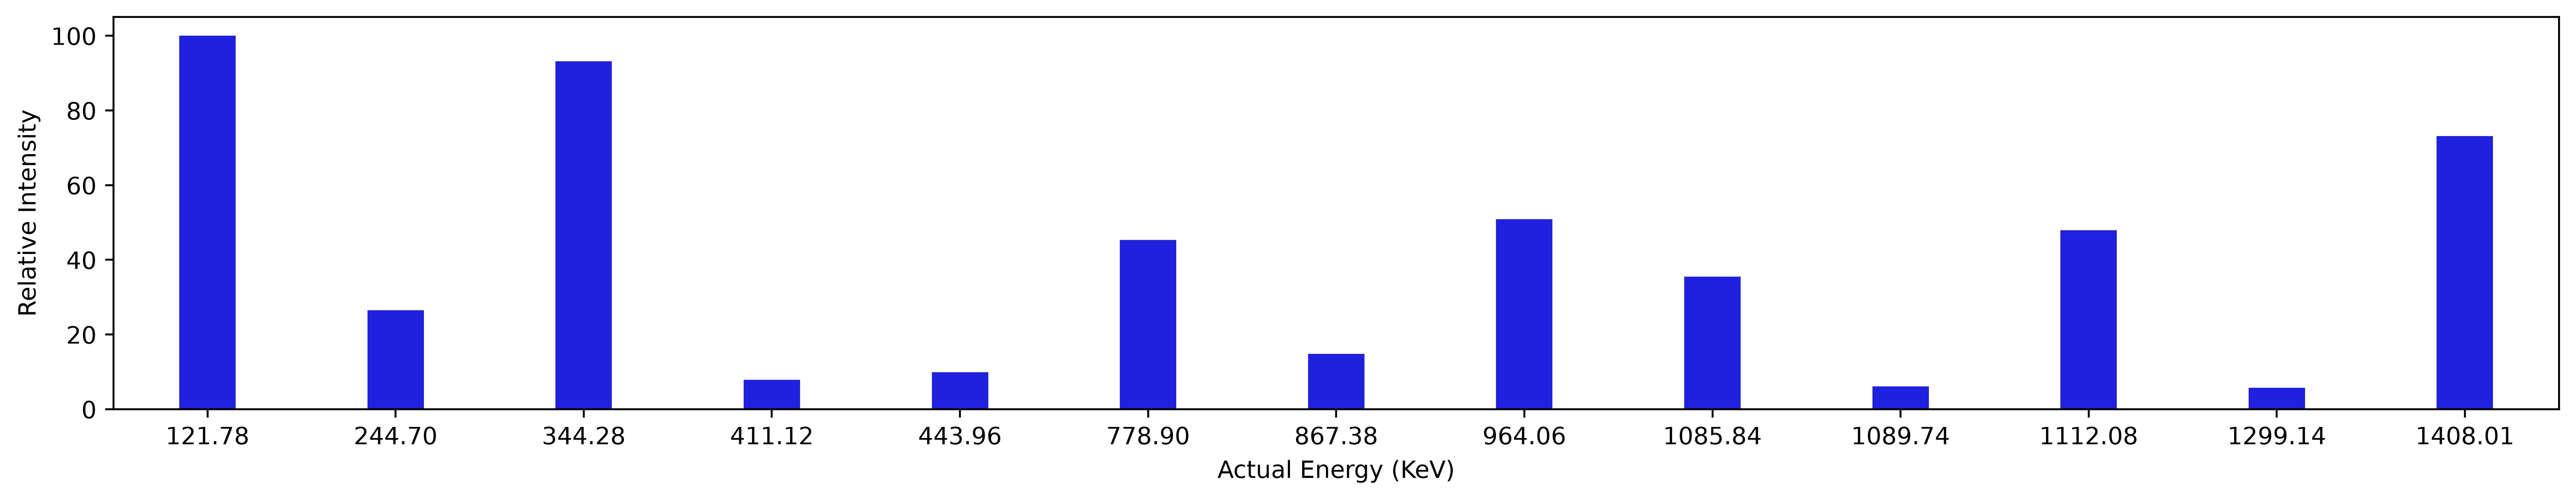
\includegraphics[width=\textwidth]{Images/actual_peaks.jpg}
	\caption{Reference gamma-ray energies from the \textbf{ENSDF} dataset. The bar height represents relative intensity.}
	\label{fig:actual energies}
\end{figure}

To identify the most suitable correspondence, we matched the measured peaks with ordered combinations of the reference energies. The ordering condition ensures that lower-positioned experimental peaks are assigned to lower-energy reference transitions, preserving the physical ordering of the spectrum.

We tested each assignment using a first-order polynomial fit and ranked the combinations according to their root-mean-square error (RMSE) as explained in the next section. We found the best-performing assignment to be the one shown in \cref{tab:calibration}.

\subsection{Determination of the Energy Calibration}
We assumed linear relationship between the measured histogram coordinate $x$ and the gamma-ray energy $E$\cite{LAVAGNO2013504}:
\begin{equation}
    E(x)=a+bx,
\end{equation}
where $a$ is the intercept and $b$ is the calibration slope. The linear coefficients were obtained using a least-squares polynomial fit to the seven assigned peak positions and their corresponding reference energies.

The quality of the linear calibration was evaluated using the root-mean-square error (RMSE), defined as
\begin{equation}
    \mathrm{RMSE}
    =\sqrt{\frac{1}{N}\sum_{i=1}^{N}
    \left(E_i-E_{\mathrm{fit},i}\right)^2}.
\end{equation}

The set of reference energies for the lowest RMSE is given in \cref{tab:calibration}. The corresponding calibration equation is
\begin{equation}
    \boxed{E(x)=-0.51337+1.19174x},
    \label{eq:calibration}
\end{equation}
where $E$ is expressed in keV and $x$ denotes the measured histogram coordinate. The RMSE is 2.9 keV.

\begin{figure}[h]
	\centering
	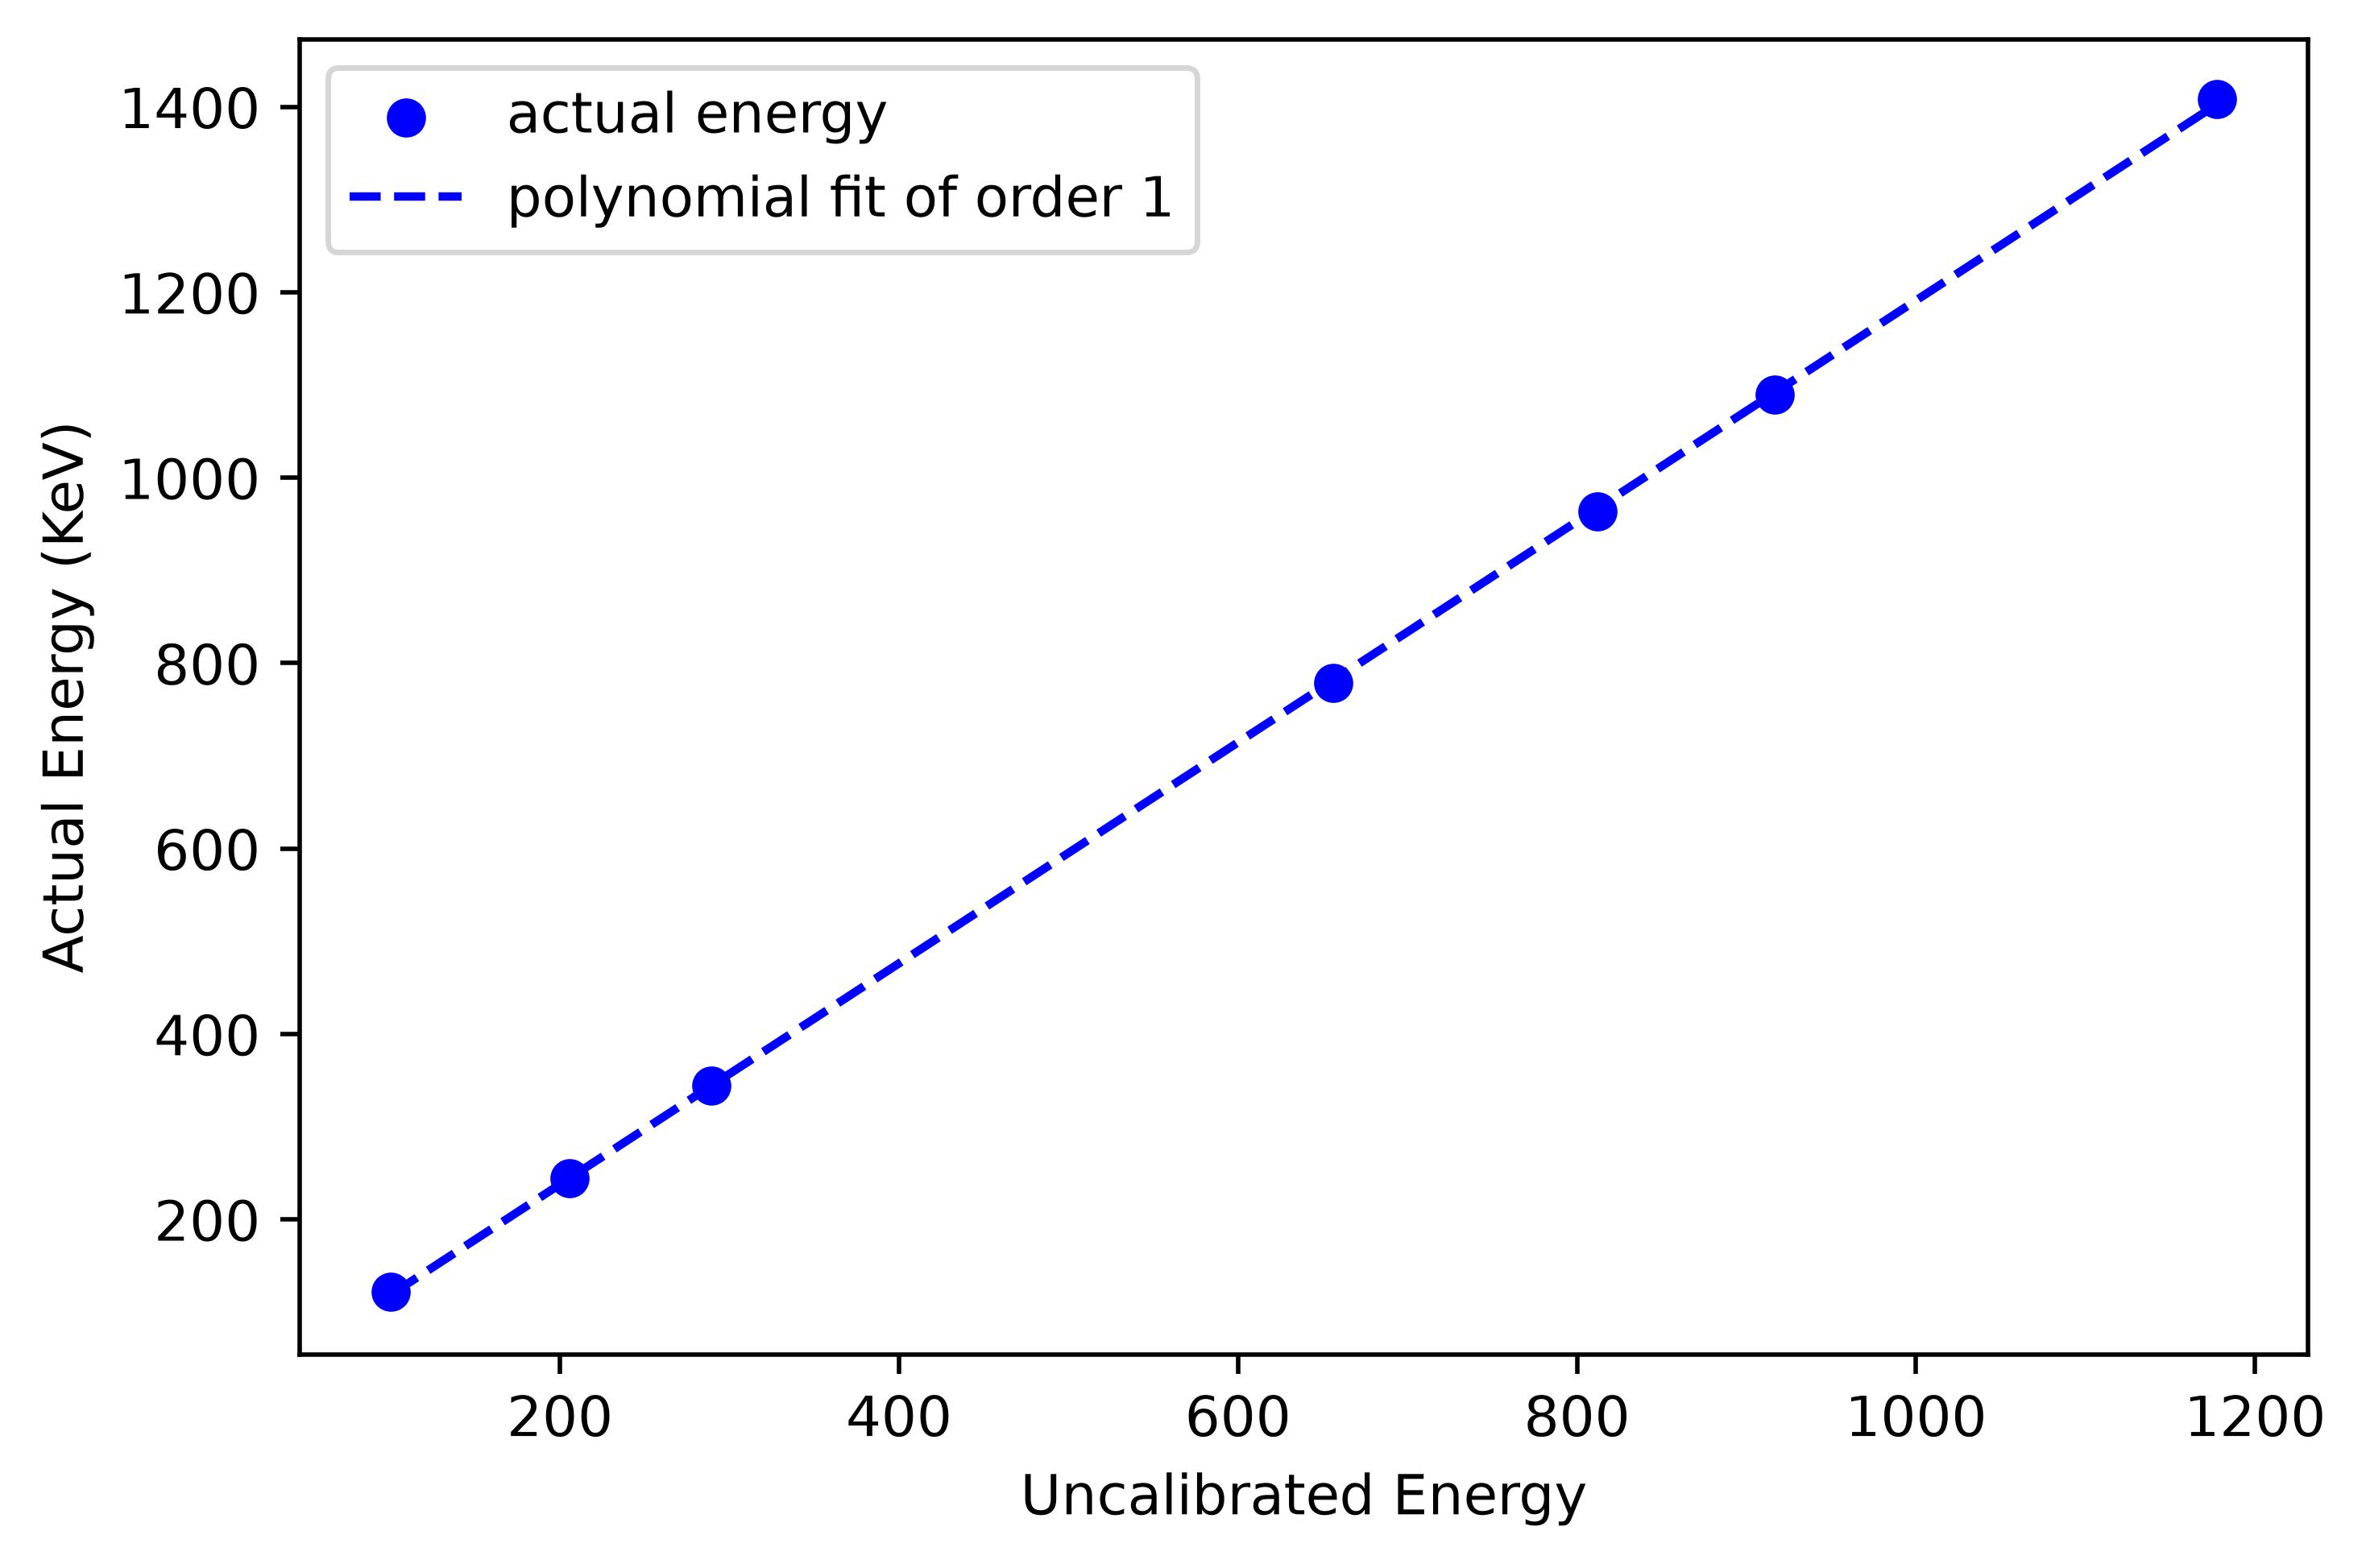
\includegraphics[width=0.7\textwidth]{Images/callibration.jpg}
	\caption{The calibration plot between the uncalibrated energies and the best matching reference energies\cref{eq:calibration}.}
	\label{fig:calibration}
\end{figure}

Using the calibration equation, the energies corresponding to the seven measured peak positions can be calculated. The residual is defined as
\begin{equation}
    \Delta E=E_{\mathrm{reference}}-E_{\mathrm{calibrated}}.
\end{equation}

\begin{table}[htbp]
    \centering
    \begin{tabular}{ccccc}
        \toprule
        Peak & Position & Reference energy (keV) & Calibrated energy (keV) & Residual (keV) \\
        \midrule
        1 & 100.21  & 121.78  & 118.91  & 2.88 \\
        2 & 205.72  & 244.70  & 244.66  & 0.04 \\
        3 & 289.30  & 344.28  & 344.26  & 0.01 \\
        4 & 656.16  & 778.90  & 781.46  & -2.55 \\
        5 & 812.19  & 964.06  & 967.41  & -3.35 \\
        6 & 916.75  & 1089.74 & 1092.02 & -2.28 \\
        7 & 1177.49 & 1408.01 & 1402.76 & 5.26 \\
        \bottomrule
    \end{tabular}
    \caption{Comparison of reference energies with the energies obtained from the linear calibration. The RMSE is 2.9 keV.}
    \label{tab:calibration}
\end{table}
